\documentclass[tikz,border=10pt]{standalone}
\usepackage{tikz}
\usetikzlibrary{shapes,arrows,positioning,calc,decorations.pathmorphing,backgrounds,shadows,fit,matrix}

% Define colors
\definecolor{primaryblue}{RGB}{0,102,204}
\definecolor{secondarygreen}{RGB}{46,204,113}
\definecolor{accentorange}{RGB}{255,127,0}
\definecolor{warningred}{RGB}{231,76,60}
\definecolor{lightgray}{RGB}{236,240,241}
\definecolor{darkgray}{RGB}{52,73,94}

\begin{document}
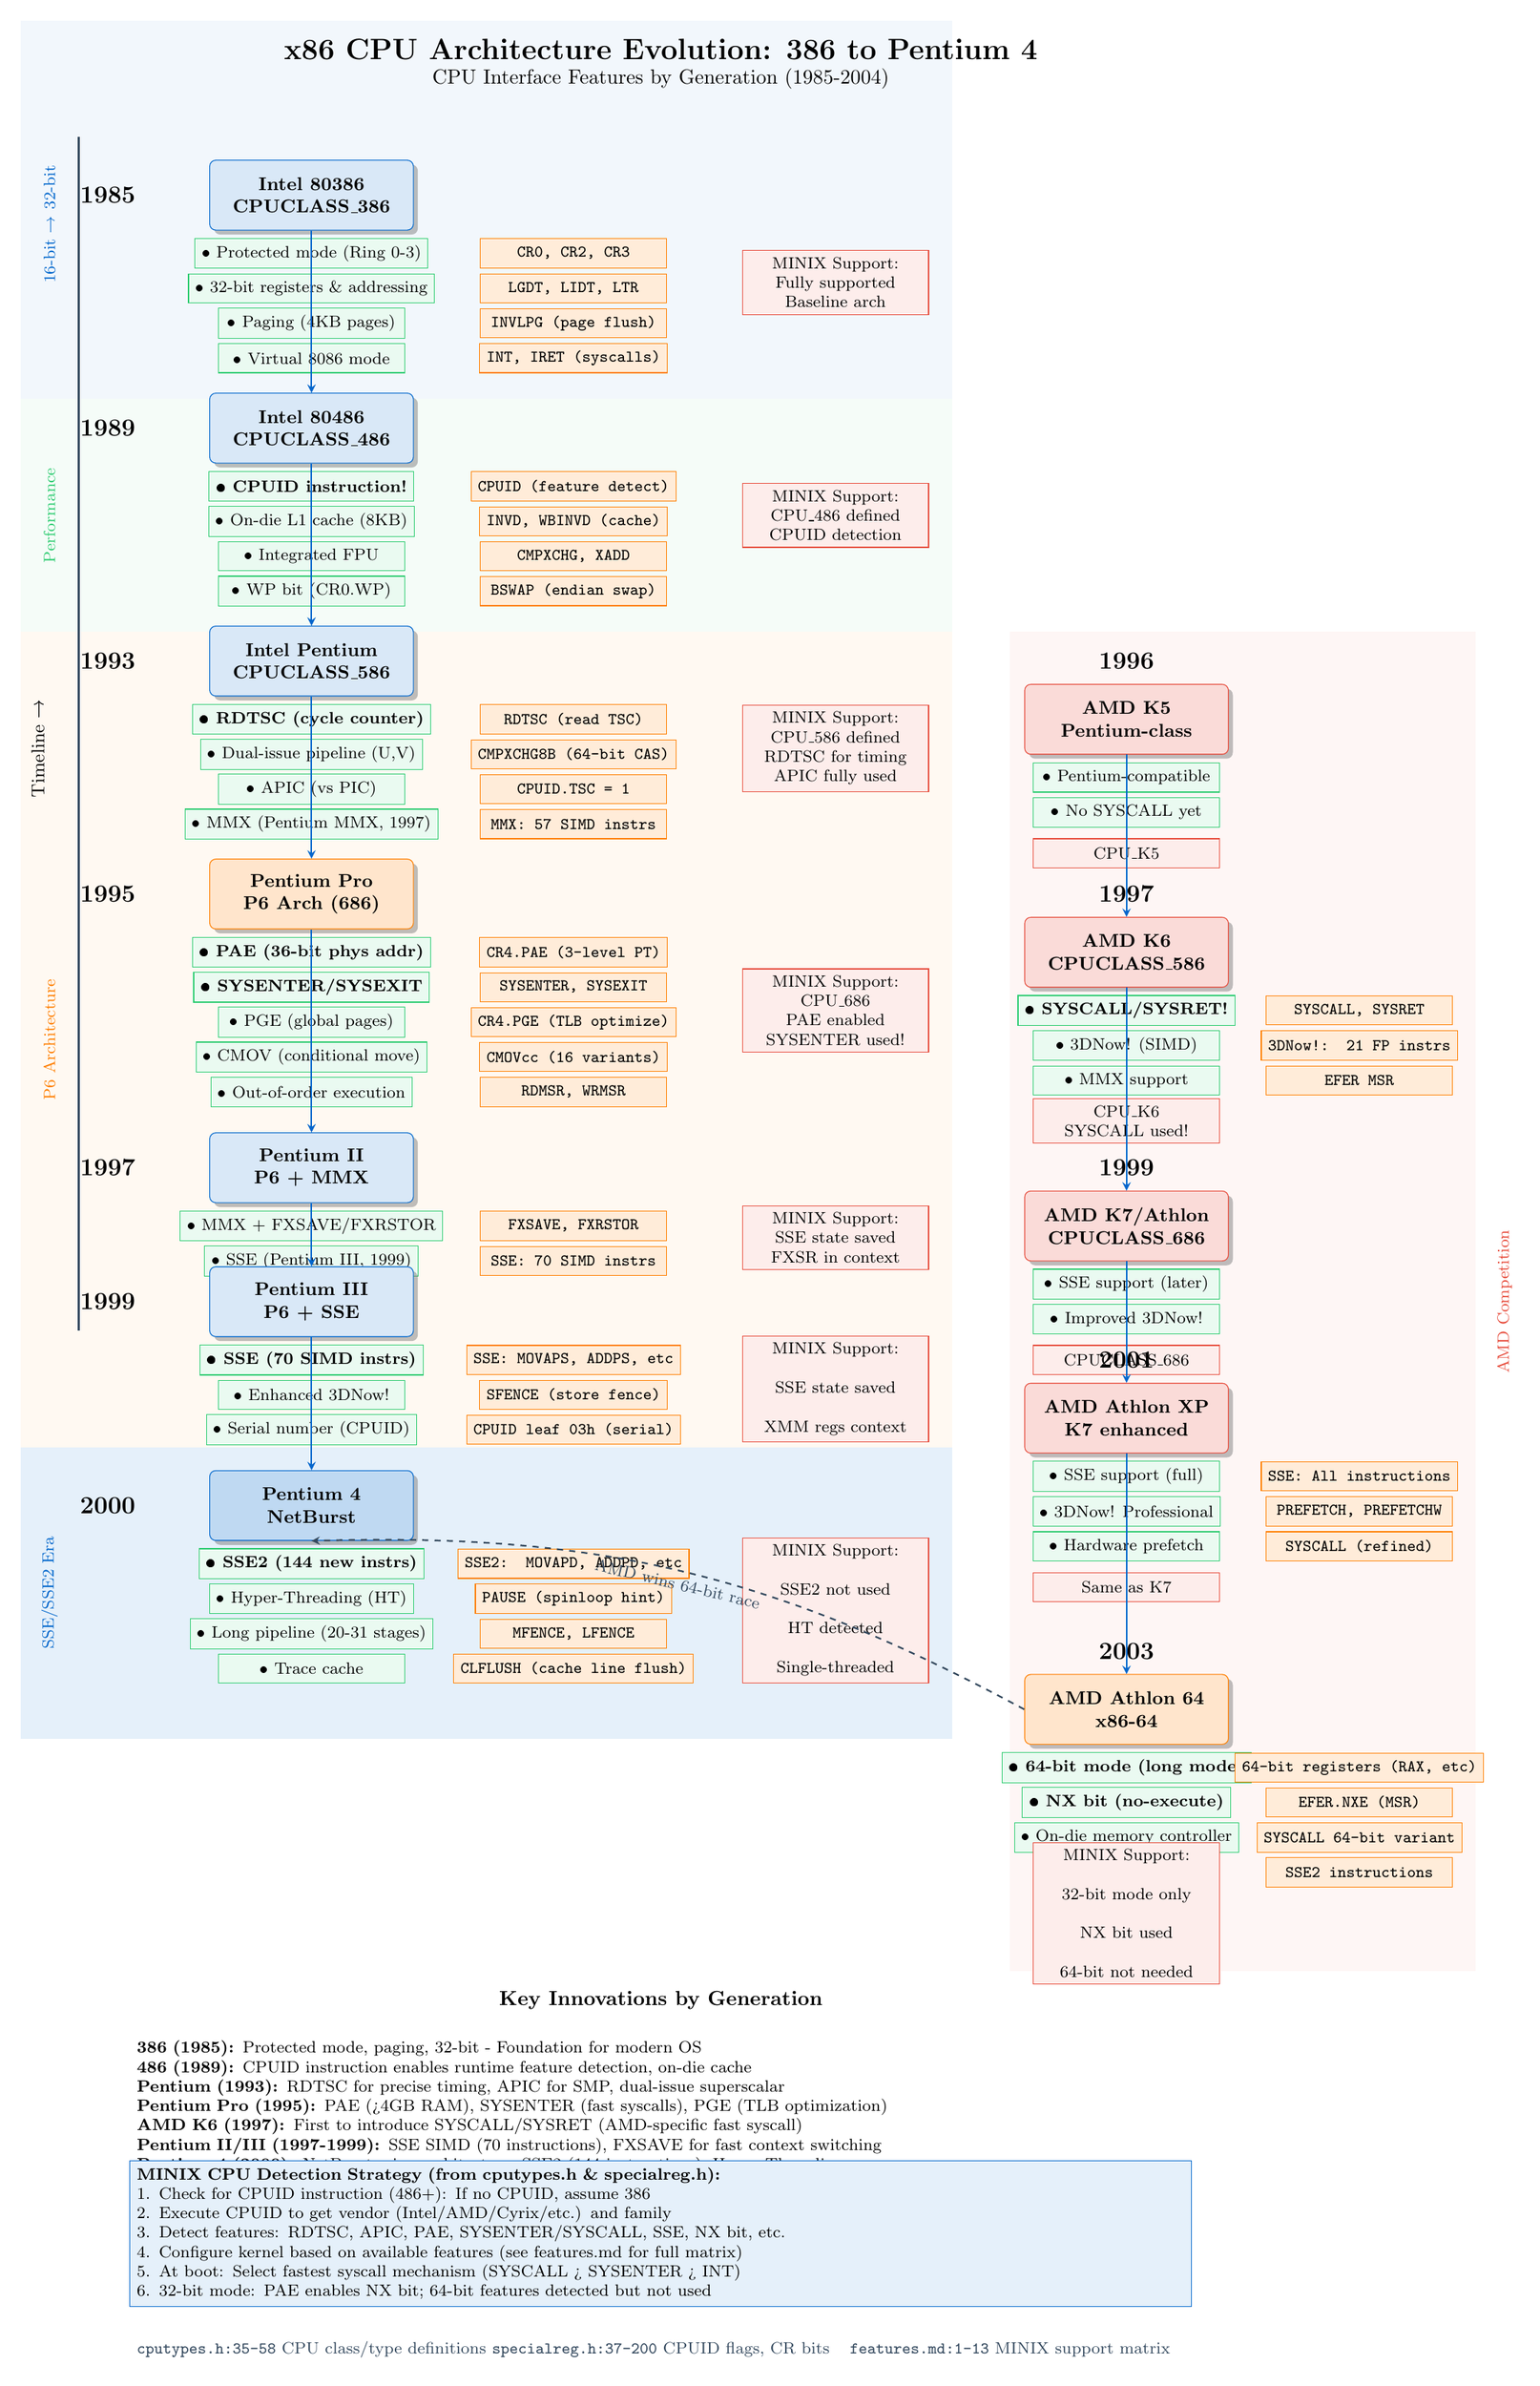
\begin{tikzpicture}[
    cpu/.style={rectangle, rounded corners=3pt, draw=primaryblue, fill=primaryblue!15, minimum width=3.5cm, minimum height=1.2cm, font=\small\bfseries, align=center, drop shadow},
    feature/.style={rectangle, draw=secondarygreen, fill=secondarygreen!10, minimum width=3.2cm, minimum height=0.5cm, font=\footnotesize, align=left},
    newinstr/.style={rectangle, draw=accentorange, fill=accentorange!15, minimum width=3.2cm, minimum height=0.5cm, font=\footnotesize\ttfamily, align=left},
    minix/.style={rectangle, draw=warningred, fill=warningred!10, minimum width=3.2cm, minimum height=0.5cm, font=\footnotesize, align=center},
    arrow/.style={->, >=stealth, thick, primaryblue},
    timeline/.style={very thick, darkgray}
]

% Title
\node[font=\Large\bfseries] at (10, 20) {x86 CPU Architecture Evolution: 386 to Pentium 4};
\node[font=\normalsize] at (10, 19.5) {CPU Interface Features by Generation (1985-2004)};

% Timeline
\draw[timeline] (0, 18.5) -- (0, -2);
\node[font=\small, rotate=90] at (-0.7, 8) {Timeline →};

%% 386 (1985)
\node[font=\bfseries\large] at (0.5, 17.5) {1985};
\node[cpu] (i386) at (4, 17.5) {Intel 80386\\CPUCLASS\_386};

\node[feature] (f386_1) at (4, 16.5) {• Protected mode (Ring 0-3)};
\node[feature] (f386_2) at (4, 15.9) {• 32-bit registers \& addressing};
\node[feature] (f386_3) at (4, 15.3) {• Paging (4KB pages)};
\node[feature] (f386_4) at (4, 14.7) {• Virtual 8086 mode};

\node[newinstr] (i386_1) at (8.5, 16.5) {CR0, CR2, CR3};
\node[newinstr] (i386_2) at (8.5, 15.9) {LGDT, LIDT, LTR};
\node[newinstr] (i386_3) at (8.5, 15.3) {INVLPG (page flush)};
\node[newinstr] (i386_4) at (8.5, 14.7) {INT, IRET (syscalls)};

\node[minix] (m386) at (13, 16) {MINIX Support:\\Fully supported\\Baseline arch};

%% 486 (1989)
\node[font=\bfseries\large] at (0.5, 13.5) {1989};
\node[cpu] (i486) at (4, 13.5) {Intel 80486\\CPUCLASS\_486};

\node[feature] (f486_1) at (4, 12.5) {\textbf{• CPUID instruction!}};
\node[feature] (f486_2) at (4, 11.9) {• On-die L1 cache (8KB)};
\node[feature] (f486_3) at (4, 11.3) {• Integrated FPU};
\node[feature] (f486_4) at (4, 10.7) {• WP bit (CR0.WP)};

\node[newinstr] (i486_1) at (8.5, 12.5) {\textbf{CPUID (feature detect)}};
\node[newinstr] (i486_2) at (8.5, 11.9) {INVD, WBINVD (cache)};
\node[newinstr] (i486_3) at (8.5, 11.3) {CMPXCHG, XADD};
\node[newinstr] (i486_4) at (8.5, 10.7) {BSWAP (endian swap)};

\node[minix] (m486) at (13, 12) {MINIX Support:\\CPU\_486 defined\\CPUID detection};

% Connection
\draw[arrow] (i386) -- (i486);

%% Pentium (1993)
\node[font=\bfseries\large] at (0.5, 9.5) {1993};
\node[cpu] (pentium) at (4, 9.5) {Intel Pentium\\CPUCLASS\_586};

\node[feature] (fp1) at (4, 8.5) {\textbf{• RDTSC (cycle counter)}};
\node[feature] (fp2) at (4, 7.9) {• Dual-issue pipeline (U,V)};
\node[feature] (fp3) at (4, 7.3) {• APIC (vs PIC)};
\node[feature] (fp4) at (4, 6.7) {• MMX (Pentium MMX, 1997)};

\node[newinstr] (ip1) at (8.5, 8.5) {\textbf{RDTSC (read TSC)}};
\node[newinstr] (ip2) at (8.5, 7.9) {CMPXCHG8B (64-bit CAS)};
\node[newinstr] (ip3) at (8.5, 7.3) {CPUID.TSC = 1};
\node[newinstr] (ip4) at (8.5, 6.7) {MMX: 57 SIMD instrs};

\node[minix] (mp) at (13, 8) {MINIX Support:\\CPU\_586 defined\\RDTSC for timing\\APIC fully used};

\draw[arrow] (i486) -- (pentium);

%% Pentium Pro (1995) - P6 Architecture
\node[font=\bfseries\large] at (0.5, 5.5) {1995};
\node[cpu, fill=accentorange!20, draw=accentorange] (ppro) at (4, 5.5) {Pentium Pro\\P6 Arch (686)};

\node[feature] (fpp1) at (4, 4.5) {\textbf{• PAE (36-bit phys addr)}};
\node[feature] (fpp2) at (4, 3.9) {\textbf{• SYSENTER/SYSEXIT}};
\node[feature] (fpp3) at (4, 3.3) {• PGE (global pages)};
\node[feature] (fpp4) at (4, 2.7) {• CMOV (conditional move)};
\node[feature] (fpp5) at (4, 2.1) {• Out-of-order execution};

\node[newinstr] (ipp1) at (8.5, 4.5) {CR4.PAE (3-level PT)};
\node[newinstr] (ipp2) at (8.5, 3.9) {\textbf{SYSENTER, SYSEXIT}};
\node[newinstr] (ipp3) at (8.5, 3.3) {CR4.PGE (TLB optimize)};
\node[newinstr] (ipp4) at (8.5, 2.7) {CMOVcc (16 variants)};
\node[newinstr] (ipp5) at (8.5, 2.1) {RDMSR, WRMSR};

\node[minix] (mpp) at (13, 3.5) {MINIX Support:\\CPU\_686\\PAE enabled\\SYSENTER used!};

\draw[arrow] (pentium) -- (ppro);

%% Pentium II (1997)
\node[font=\bfseries\large] at (0.5, 0.8) {1997};
\node[cpu] (p2) at (4, 0.8) {Pentium II\\P6 + MMX};

\node[feature] (fp2_1) at (4, -0.2) {• MMX + FXSAVE/FXRSTOR};
\node[feature] (fp2_2) at (4, -0.8) {• SSE (Pentium III, 1999)};

\node[newinstr] (ip2_1) at (8.5, -0.2) {FXSAVE, FXRSTOR};
\node[newinstr] (ip2_2) at (8.5, -0.8) {SSE: 70 SIMD instrs};

\node[minix] (mp2) at (13, -0.4) {MINIX Support:\\SSE state saved\\FXSR in context};

\draw[arrow] (ppro) -- (p2);

% Right column: AMD processors

%% AMD K5 (1996)
\node[font=\bfseries\large] at (18, 9.5) {1996};
\node[cpu, fill=warningred!20, draw=warningred] (k5) at (18, 8.5) {AMD K5\\Pentium-class};

\node[feature] (fk5_1) at (18, 7.5) {• Pentium-compatible};
\node[feature] (fk5_2) at (18, 6.9) {• No SYSCALL yet};

\node[minix] (mk5) at (18, 6.2) {CPU\_K5};

%% AMD K6 (1997)
\node[font=\bfseries\large] at (18, 5.5) {1997};
\node[cpu, fill=warningred!20, draw=warningred] (k6) at (18, 4.5) {AMD K6\\CPUCLASS\_586};

\node[feature] (fk6_1) at (18, 3.5) {\textbf{• SYSCALL/SYSRET!}};
\node[feature] (fk6_2) at (18, 2.9) {• 3DNow! (SIMD)};
\node[feature] (fk6_3) at (18, 2.3) {• MMX support};

\node[newinstr] (ik6_1) at (22, 3.5) {\textbf{SYSCALL, SYSRET}};
\node[newinstr] (ik6_2) at (22, 2.9) {3DNow!: 21 FP instrs};
\node[newinstr] (ik6_3) at (22, 2.3) {EFER MSR};

\node[minix] (mk6) at (18, 1.6) {CPU\_K6\\SYSCALL used!};

\draw[arrow] (k5) -- (k6);

%% AMD K7/Athlon (1999)
\node[font=\bfseries\large] at (18, 0.8) {1999};
\node[cpu, fill=warningred!20, draw=warningred] (k7) at (18, -0.2) {AMD K7/Athlon\\CPUCLASS\_686};

\node[feature] (fk7_1) at (18, -1.2) {• SSE support (later)};
\node[feature] (fk7_2) at (18, -1.8) {• Improved 3DNow!};

\node[minix] (mk7) at (18, -2.5) {CPUCLASS\_686};

\draw[arrow] (k6) -- (k7);

%% Pentium III (1999)
\node[font=\bfseries\large] at (0.5, -1.5) {1999};
\node[cpu] (p3) at (4, -1.5) {Pentium III\\P6 + SSE};

\node[feature] (fp3_1) at (4, -2.5) {\textbf{• SSE (70 SIMD instrs)}};
\node[feature] (fp3_2) at (4, -3.1) {• Enhanced 3DNow!};
\node[feature] (fp3_3) at (4, -3.7) {• Serial number (CPUID)};

\node[newinstr] (ip3_1) at (8.5, -2.5) {\textbf{SSE: MOVAPS, ADDPS, etc}};
\node[newinstr] (ip3_2) at (8.5, -3.1) {SFENCE (store fence)};
\node[newinstr] (ip3_3) at (8.5, -3.7) {CPUID leaf 03h (serial)};

\node[minix] (mp3) at (13, -3) {MINIX Support:\\\\SSE state saved\\\\XMM regs context};

\draw[arrow] (p2) -- (p3);

%% Pentium 4 (2000)
\node[font=\bfseries\large] at (0.5, -5) {2000};
\node[cpu, fill=primaryblue!25, draw=primaryblue] (p4) at (4, -5) {Pentium 4\\NetBurst};

\node[feature] (fp4_1) at (4, -6) {\textbf{• SSE2 (144 new instrs)}};
\node[feature] (fp4_2) at (4, -6.6) {• Hyper-Threading (HT)};
\node[feature] (fp4_3) at (4, -7.2) {• Long pipeline (20-31 stages)};
\node[feature] (fp4_4) at (4, -7.8) {• Trace cache};

\node[newinstr] (ip4_1) at (8.5, -6) {SSE2: MOVAPD, ADDPD, etc};
\node[newinstr] (ip4_2) at (8.5, -6.6) {PAUSE (spinloop hint)};
\node[newinstr] (ip4_3) at (8.5, -7.2) {MFENCE, LFENCE};
\node[newinstr] (ip4_4) at (8.5, -7.8) {CLFLUSH (cache line flush)};

\node[minix] (mp4) at (13, -6.8) {MINIX Support:\\\\SSE2 not used\\\\HT detected\\\\Single-threaded};

\draw[arrow] (p3) -- (p4);

%% AMD Athlon XP (2001)
\node[font=\bfseries\large] at (18, -2.5) {2001};
\node[cpu, fill=warningred!20, draw=warningred] (axp) at (18, -3.5) {AMD Athlon XP\\K7 enhanced};

\node[feature] (faxp_1) at (18, -4.5) {• SSE support (full)};
\node[feature] (faxp_2) at (18, -5.1) {• 3DNow! Professional};
\node[feature] (faxp_3) at (18, -5.7) {• Hardware prefetch};

\node[newinstr] (iaxp_1) at (22, -4.5) {SSE: All instructions};
\node[newinstr] (iaxp_2) at (22, -5.1) {PREFETCH, PREFETCHW};
\node[newinstr] (iaxp_3) at (22, -5.7) {SYSCALL (refined)};

\node[minix] (maxp) at (18, -6.4) {Same as K7};

\draw[arrow] (k7) -- (axp);

%% AMD Athlon 64 (2003)
\node[font=\bfseries\large] at (18, -7.5) {2003};
\node[cpu, fill=accentorange!20, draw=accentorange] (a64) at (18, -8.5) {AMD Athlon 64\\x86-64};

\node[feature] (fa64_1) at (18, -9.5) {\textbf{• 64-bit mode (long mode)}};
\node[feature] (fa64_2) at (18, -10.1) {\textbf{• NX bit (no-execute)}};
\node[feature] (fa64_3) at (18, -10.7) {• On-die memory controller};
\node[feature] (fa64_4) at (18, -11.3) {• SSE2 support};

\node[newinstr] (ia64_1) at (22, -9.5) {64-bit registers (RAX, etc)};
\node[newinstr] (ia64_2) at (22, -10.1) {\textbf{EFER.NXE (MSR)}};
\node[newinstr] (ia64_3) at (22, -10.7) {SYSCALL 64-bit variant};
\node[newinstr] (ia64_4) at (22, -11.3) {SSE2 instructions};

\node[minix] (ma64) at (18, -12) {MINIX Support:\\\\32-bit mode only\\\\NX bit used\\\\64-bit not needed};

\draw[arrow] (axp) -- (a64);

% Connection AMD to Intel (64-bit race)
\draw[arrow, dashed, darkgray] (a64.west) to[bend right=15] node[below, sloped, font=\footnotesize] {AMD wins 64-bit race} (p4.south);

% Background zones (extended)
\begin{scope}[on background layer]
    \fill[primaryblue!5] (-1, 20.5) rectangle (15, 14);
    \fill[secondarygreen!5] (-1, 14) rectangle (15, 10);
    \fill[accentorange!5] (-1, 10) rectangle (15, -4);
    \fill[primaryblue!10] (-1, -4) rectangle (15, -9);
    \fill[warningred!5] (16, 10) rectangle (24, -13);
\end{scope}

% Zone labels
\node[font=\footnotesize, rotate=90, primaryblue] at (-0.5, 17) {16-bit → 32-bit};
\node[font=\footnotesize, rotate=90, secondarygreen] at (-0.5, 12) {Performance};
\node[font=\footnotesize, rotate=90, accentorange] at (-0.5, 3) {P6 Architecture};
\node[font=\footnotesize, rotate=90, primaryblue] at (-0.5, -6.5) {SSE/SSE2 Era};
\node[font=\footnotesize, rotate=90, warningred] at (24.5, -1.5) {AMD Competition};

% Legend
\node[font=\bfseries] at (10, -13.5) {Key Innovations by Generation};
\node[font=\footnotesize, align=left, text width=18cm] at (10, -15.5) {
\textbf{386 (1985):} Protected mode, paging, 32-bit - Foundation for modern OS\\
\textbf{486 (1989):} CPUID instruction enables runtime feature detection, on-die cache\\
\textbf{Pentium (1993):} RDTSC for precise timing, APIC for SMP, dual-issue superscalar\\
\textbf{Pentium Pro (1995):} PAE (>4GB RAM), SYSENTER (fast syscalls), PGE (TLB optimization)\\
\textbf{AMD K6 (1997):} First to introduce SYSCALL/SYSRET (AMD-specific fast syscall)\\
\textbf{Pentium II/III (1997-1999):} SSE SIMD (70 instructions), FXSAVE for fast context switching\\
\textbf{Pentium 4 (2000):} NetBurst microarchitecture, SSE2 (144 instructions), Hyper-Threading\\
\textbf{AMD Athlon 64 (2003):} First x86-64 implementation, NX bit for DEP, on-die memory controller
};

% MINIX detection note
\node[rectangle, draw=primaryblue, fill=primaryblue!10, text width=18cm, align=left, font=\footnotesize] at (10, -17.5) {
\textbf{MINIX CPU Detection Strategy (from cputypes.h \& specialreg.h):}\\
1. Check for CPUID instruction (486+): If no CPUID, assume 386\\
2. Execute CPUID to get vendor (Intel/AMD/Cyrix/etc.) and family\\
3. Detect features: RDTSC, APIC, PAE, SYSENTER/SYSCALL, SSE, NX bit, etc.\\
4. Configure kernel based on available features (see features.md for full matrix)\\
5. At boot: Select fastest syscall mechanism (SYSCALL > SYSENTER > INT)\\
6. 32-bit mode: PAE enables NX bit; 64-bit features detected but not used
};

% File references
\node[font=\footnotesize, text=darkgray] at (4, -19.5) {
\texttt{cputypes.h:35-58} CPU class/type definitions
};

\node[font=\footnotesize, text=darkgray] at (10, -19.5) {
\texttt{specialreg.h:37-200} CPUID flags, CR bits
};

\node[font=\footnotesize, text=darkgray] at (16, -19.5) {
\texttt{features.md:1-13} MINIX support matrix
};

\end{tikzpicture}
\end{document}
